\section{Vertex-Centric Graph Index}\label{sec:storage}
\begin{figure*}
  \centering
  \begin{subfigure}[b]{0.27\textwidth}
    \centering
    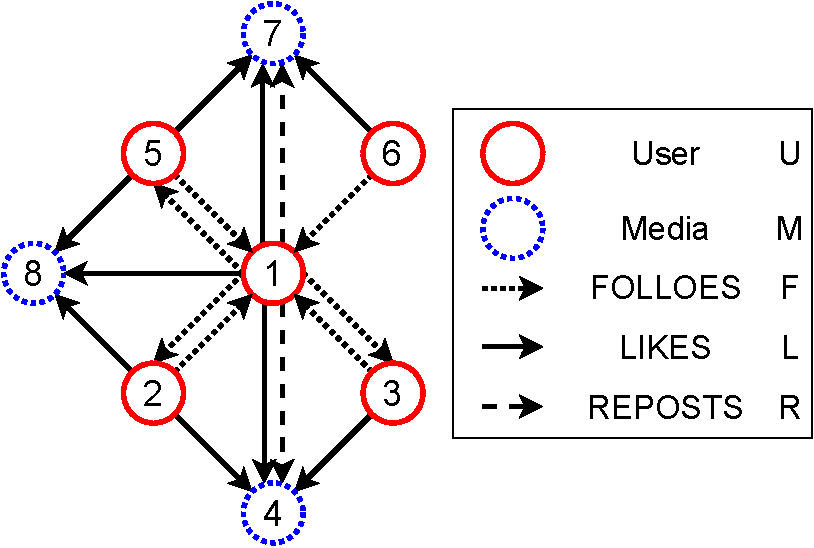
\includegraphics[scale=0.4]{img/data_graph}
    \caption{Data graph.}\label{fig:data_graph}
  \end{subfigure}
  \quad
  \begin{minipage}[b]{0.68\textwidth}
    \centering
    \begin{subfigure}[b]{\textwidth}
      \centering
      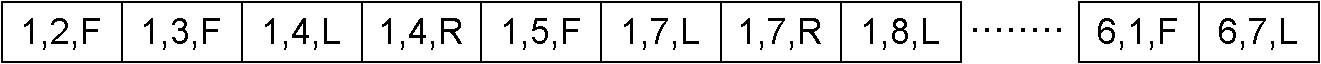
\includegraphics[scale=0.3]{img/data_edge}
      \caption{Edge List.}\label{fig:data_edge}
    \end{subfigure}
    \\
    \begin{subfigure}[b]{0.35\textwidth}
      \centering
      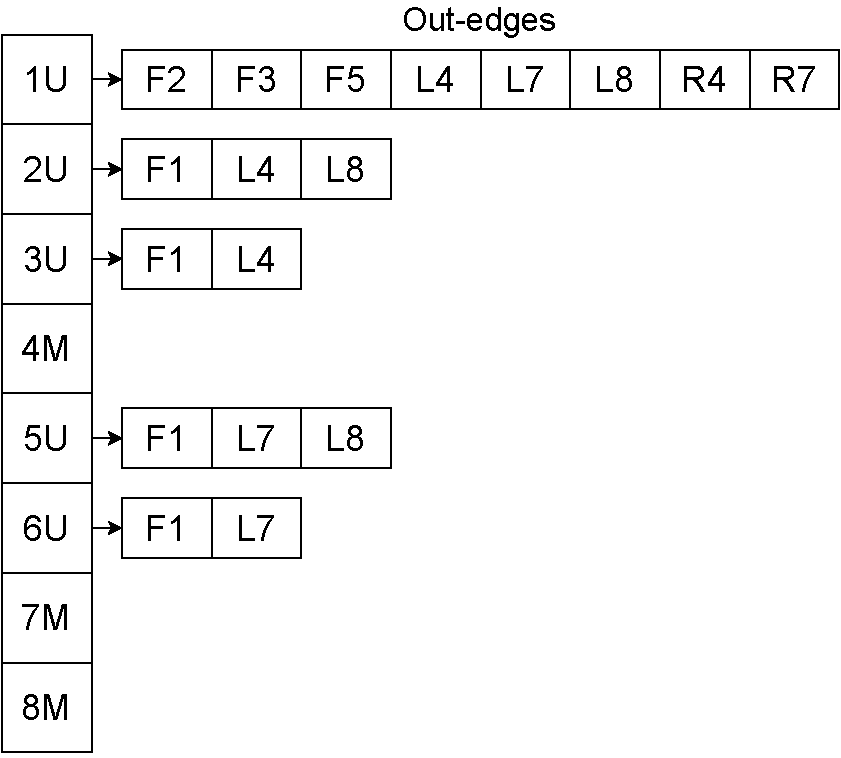
\includegraphics[scale=0.3]{img/data_row}
      \caption{Row-based.}\label{fig:data_row}
    \end{subfigure}
    \quad
    \begin{subfigure}[b]{0.2\textwidth}
      \centering
      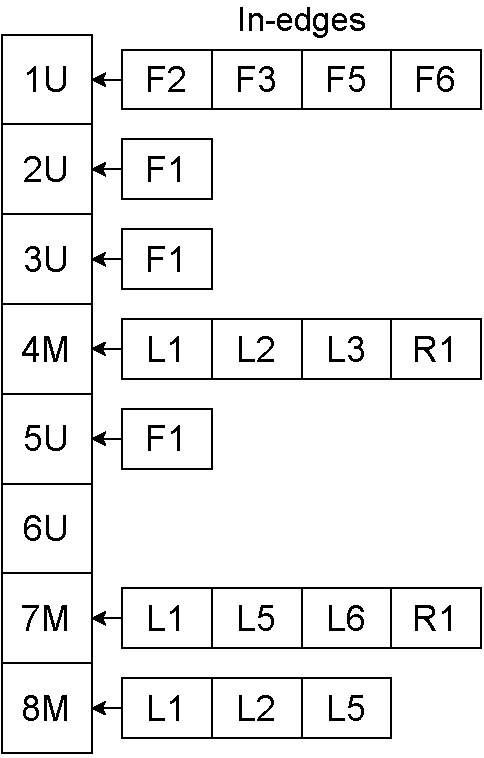
\includegraphics[scale=0.3]{img/data_column}
      \caption{Column-based.}\label{fig:data_column}
    \end{subfigure}
    \quad
    \begin{subfigure}[b]{0.3\textwidth}
      \centering
      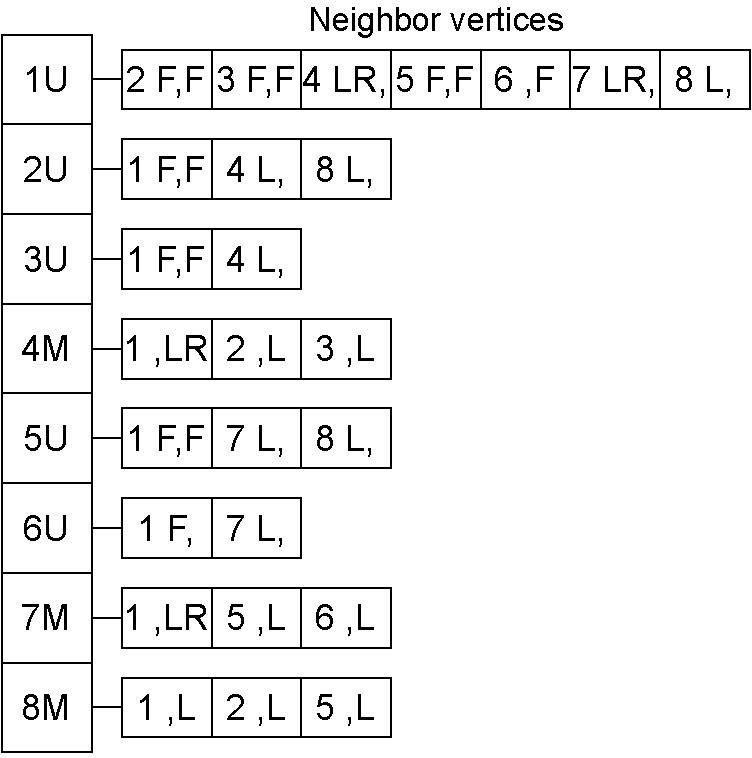
\includegraphics[scale=0.3]{img/data_vertex_centric}
      \caption{Vertex-centric.}\label{fig:data_vertex_centric}
    \end{subfigure}
  \end{minipage}
  \caption{Sample data graph and its various storage methods.}\label{img:data}
\end{figure*}
A data structure is a way to store and organize data in order to facilitates access and modifications~\cite{DBLP:books/daglib/0023376}.
The performance of a graph matching algorithm is closely related to its storing structure.
This section first shows the opportunities by studying existing graph storage methods,
then presents the design of SeqStar's graph index.

\subsection{Opportunities}
A graph can be represented by its adjacency matrix~\cite{DBLP:books/sp/BondyM08}.
Based on the accessing order of the matrix, existing graph storage methods can be categorized into three types:
\emph{edges list}, \emph{row-based} and \emph{column-based}.

Consider the sample data graph in Figure~\ref{fig:data_graph}, the \emph{edge list} format stores each edge and its corresponding source and destination vertices as a sequence (Figure~\ref{fig:data_edge}).
In the language of linear algebra, edge list is known as \emph{coordinate list (COO)}, which stores a list of $(row, column, value)$ tuples.
However, the neighbors of each vertex are scattered across in edge list~\cite{DBLP:conf/fast/KumarH19}, thus is not an optimal choice for graph matching problems.

In order to access the in/out-edges of each vertex efficiently, the edge list is partitioned by the destination/source vertices.
\emph{Row-based} format can access the out-edges of a vertex efficiently.
As is shown in Figure~\ref{fig:data_row}, out-edges are grouped by the sources.
The physical structure of the row-based format can be either \emph{array based} or \emph{linked list based}.
The compressed sparse row (CSR) format stores the out-edges consecutively in an array, and use a vertex array to store the offset and size for each vertex.
Whereas the adjacency list structure stores the out-edges of each vertex separately.
Array based structure has better locality and is more suitable for graph analysis problems, whereas linked list structure are good at updates.
\emph{Column-based} format partitions the in-edges by the destinations (Figure~\ref{fig:data_column}).
Similar to the row-based format, the physical structure of column-based format can also be array/linked list based.

Graph problems are notorious for their high data access to computation ratio~\cite{DBLP:journals/ppl/LumsdaineGHB07}.
As a result, the storage of graphs plays an important part in the workflow.

\subsection{Vertex-Centric Storage Model}

\subsection{Global/Local Indexes}
